\section{Semantische Tableaus}
Die Methode der semantischen Tableaus ist eine effiziente Entscheidungsprozedur für Erfüllbarkeit (und Dualität) in der Aussagenlogik.

Das Prinzip hinter semantischen Tableaus ist sehr einfach: Sucht man nach einem Modell, das die Interpretation erfüllt, indem man die Formel in Atommengen und Atomnegationen zerlegt. Es ist leicht zu überprüfen, ob es für jede Menge eine Interpretation gibt: Eine Menge von Atomen und Negationen von Atomen ist erfüllbar, wenn die Menge kein Atom p und seine Negation $\neg$p enthält. Die Formel ist erfüllbar, wenn eine dieser Mengen erfüllbar ist.

\subsection{Zerlegen von Formeln in Sätze von Literalen}

\begin{defi} \label{Definition 2.57} \end{defi} Ein Literal ist ein Atom oder die Negation eines Atoms. Ein Atom ist ein positives Literal und die Negation eines Atoms ist ein negatives Literal. Für jedes Atom $p$ ist $\{p, \neg p\}$ ein komplementäres Literalpaar.

Für jede Formel $A$ ist $\{A, \neg A\}$ ein komplementäres Formelpaar. A ist das Komplement von $\neg A$ und $\neg A$ ist das Komplement von A.

\begin{ex} \label{Beispiel 2.58} \end{ex} In der Menge der Literale $ \{ \neg p, q, r, \neg r \} $ sind q und r positive Literale, während $\neg p$ und $\neg r$ negative Literale sind. Die Menge enthält das komplementäre Literalpaar $ \{ r, \neg r \}$.
 
\begin{sa} \label{Satz 2.60 } \end{sa}Eine Menge von Literalen ist genau dann erfüllbar, wenn sie vorhanden ist
enthält kein komplementäres Literalpaar.


\subsection{Konstruktion von semantischen Tableaus}
In der Methode der semantischen Tableaus bezeichnen Mengen von Formeln Knoten eines Baumes, wobei jeder Pfad im Baum die Formeln darstellt, die in einer möglichen Interpretation erfüllt sein müssen.

Die Anfangsformel kennzeichnet die Wurzel des Baumes. Jeder Knoten hat einen oder zwei untergeordnete Knoten, abhängig davon, wie eine Formel, die den Knoten kennzeichnet, zerlegt wird. Die Blätter sind durch die Literale gekennzeichnet. Ein Blatt, das durch eine Menge von Literalen markiert ist, die ein komplementäres Paar von Literalen enthalten, ist mit $\times$ markiert, während ein Blatt, das durch eine Menge markiert ist, die kein komplementäres Paar enthält, mit $\odot$ markiert ist.

Abbildung \ref{Abb. 2.7} zeigt semantische Tableaus für die Formeln:\\
$A = p\wedge (\neg q \vee \neg p)$ und $B = (p \vee q) \wedge  (\neg p \wedge  \neg q)$.

\begin{figure}[ !h] \centering											
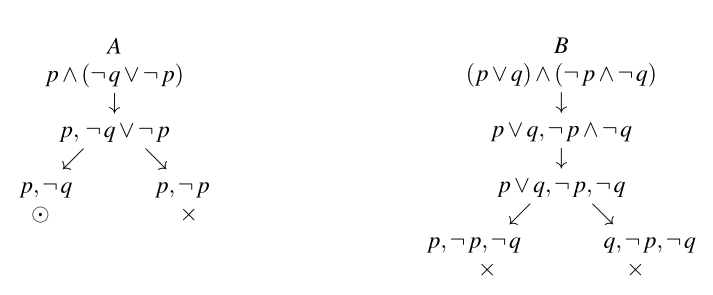
\includegraphics[width=1.0\textwidth]{A25}
\caption[Semantische Tableaus]{Semantische Tableaus}
\label{Abb. 2.7}
\end{figure}

Die Tableau-Konstruktion ist nicht eindeutig; Hier ist ein weiteres Tableau für $B$:

\begin{figure}[ !h] \centering												
 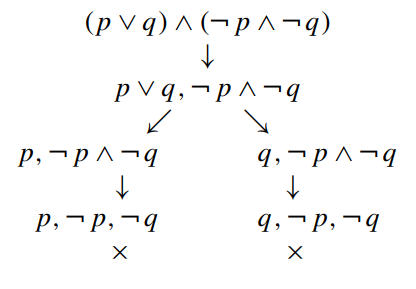
\includegraphics[width=0.5\textwidth]{A26}	
 \label{Abb. A26}
\end{figure}

%\begin{figure}[ !h] \centering											
%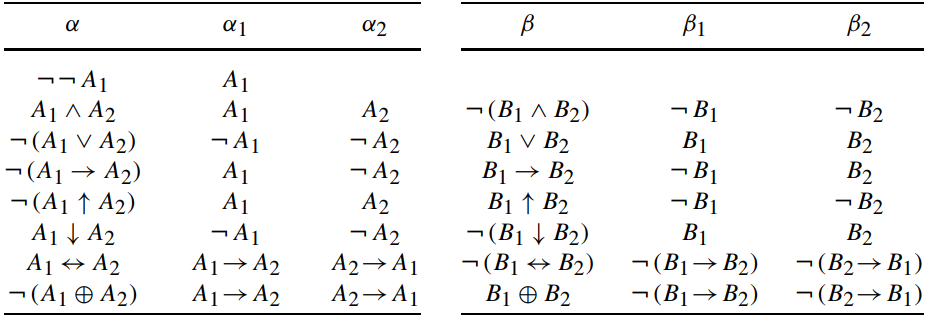
\includegraphics[width=1.0\textwidth]{A27}
%\caption[ Klassifizierung von $\alpha$- und $\beta$-Formeln]{ Klassifizierung von $\alpha$- und $\beta$-Formeln}
%\label{Abb. 2.8}
%\end{figure}

\begin{table}[h]
\footnotesize
	\begin{center}
			\begin{tabular}{ccccccc}
			\cline{1-3}
			\cline{5-7}
			$\alpha$  & $\alpha_1$ & $\alpha_2$ &   &$\beta$&$\beta_1$&$\beta_2$  \\
			\cline{1-3} 
			\cline{5-7}
			
			$\neg \neg A_1$  & $A_1$ &  &   &&& \\
			
			$A_1 \wedge A_2$  & $A_1$ & $A_2$ &   &$\neg (B_1 \wedge B_2$&$\neg B_1$&$\neg B_2$  \\
			
			$\neg (A_1 \vee A_2)$  & $\neg A_1$ & $\neg A_2$ &   &$B_1 \vee B_2 $&$B_1$&$B_2$  \\
			
			$\neg (A_1 \rightarrow A_2)$  & $A_1$ & $\neg A_2$ &   &$B_1 \rightarrow B_2)$&$\neg B_1$&$B_2$  \\
			
			$\neg(A_1 \uparrow A_2)$  & $A_1$ & $A_2$ &   &$B_1 \uparrow B_2$&$\neg B_1$&$\neg B_2$  \\
			
			$A_1 \downarrow A_2$  & $\neg A_1$ & $\neg A_2$ &   &$\neg (B_1 \downarrow B_2)$&$B_1$&$B_2$  \\
			
			$A_1 \leftrightarrow A_2$  & $A_1 \rightarrow A_2$ & $A_2 \rightarrow A_1$ &   &$\neg (B_1 \leftrightarrow B_2)$&$\neg (B_1 \rightarrow B_2)$&$\neg (B_2 \rightarrow B_1)$  \\
			
			$\neg (A_1 \oplus A_2)$  & $A_1 \rightarrow A_2$ & $A_2 \rightarrow A_1$ &   &$B_1 \oplus B_2$&$\neg (B_1 \rightarrow B_2)$&$\neg (B_2 \rightarrow B_1)$  \\
			\cline{1-3} 
			\cline{5-7}
			\end{tabular}
	\end{center}
	\caption[$\alpha$- und $\beta$-Formeln]{Klassifizierung von $\alpha$- und $\beta$-Formeln}
	\label{Abb. 2.8}
\end{table}			

Es wird durch Verzweigen konstruiert, um nach einer befriedigenden Belegung für $p \vee q$ zu suchen, bevor nach einem für $\neg p \wedge \neg q$ gesucht wird. Das erste Tableau enthält weniger Knoten, was zeigt, dass es vorzuziehen ist, \textit{Konjunktionen vor Disjunktionen} zu zerlegen.

Eine übersichtliche Darstellung der Regeln für die Erstellung eines semantischen Tableaus kann gegeben werden, wenn \textit{Formeln nach ihrem Hauptoperator klassifiziert} werden (Tabelle \ref{Abb. 2.8}). Wenn \textit{die Formel eine Negation ist, berücksichtigt die Klassifizierung sowohl die Negation als auch den Hauptoperator}. \textit{$\alpha$-Formeln sind Konjunktiv} und nur erfüllbar, wenn beide Teilformeln $\alpha$1 und $\alpha$2 erfüllt sind, während \textit{$\beta$-Formeln disjunktiv sind} und auch dann erfüllt sind, wenn nur eine der Teilformeln $\beta$1 oder $\beta$2 erfüllbar ist.

\begin{ex} \label{Beispiel 2.63} \end{ex} Die Formel p $\in$ q wird als $\alpha$ -Formel klassifiziert, weil sie genau dann gilt, wenn sowohl p als auch q wahr sind. Die Formel $\neg$ (p$\wedge$ q) wird als $\beta$-Formel klassifiziert.
Es ist logisch äquivalent zu $\neg$p $\vee$ $\neg$q und ist genau dann wahr, wenn entweder $\neg$p wahr oder $\neg$q wahr ist.

\begin{al}Konstruktion eines semantischen Tableaus \label{Algorithmus 2.64} \end{al} 
\begin{tabbing}  
\hspace{0.3in} \= \hspace{0.3in} \=  \hspace{0.3in} \= \hspace{0.3in} \= \kill
Eingabe: Aussagenlogische Formel $A$.\\
Ausgabe: Semantisches Tableau mit markierten Blättern\\
\textbf{function} Tableau(A)\\
\> Konstruiere einen Baum mit Formel $A$ als Wurzel.\\
\> \textbf{while} es gibt unmarkierte Blätter \textbf{do} \\
\> Wähle unmarkiertes Blatt $l$\\
\> \>\textbf{if}  Blatt $l$ enthält nur Literale then\\
\> \> \> if Blatt l enthält komplementäre Literale then\\
\> \> \> \> Markiere Blatt $l$ als geschlossen mit $\times$ \\
\> \> \> \textbf{else} \\
\> \> \> \> Markiere Blatt $l$ als offen mit\\
\> \> \> \textbf{end if} \\
\> \> \textbf{else if}  Blatt $l$ enthält $\alpha$-Formel then\\
\> \> \> Wähle $\alpha$-Formel $\alpha$\\
\>\>\> Ermittle Formeln $\alpha_1$ und $\alpha_2$ nach Tabelle \ref{Abb. 2.8}\\
\>\>\> Erzeuge Kind $l´$ von $l$\\
\>\>\> Beschrifte $l´$ mit Formeln aus $l$\\
\>\>\> Ersetze dabei $\alpha$ in $l´$ durch Formeln $\alpha_1$  und $\alpha_2$\\
\>\> \textbf{else} \\
\>\>\> Wähle b-Formel $\beta$\\
\>\>\> Ermittle Formeln $\beta_1$ und $\beta_2$ nach Tabelle \ref{Abb. 2.8}\\
\>\>\> Erzeuge zwei Kinder $l_1$ und $l_2$ von $l$\\
\>\>\> Beschrifte $l_1$ mit Formeln aus $l$\\
\>\>\> Ersetze dabei $\beta$ in $l_1$ durch $\beta_1$\\
\>\>\> Beschrifte $l_2$ mit Formeln aus $l$\\
\>\>\> Ersetze dabei $\beta$ in $l_2$ durch $\beta_2$\\
\>\> \textbf{end if} \\
\> \textbf{end while} \\
\> \textbf{return}  Semantisches Tableau\\
\textbf{end function} \\
\end{tabbing} 

\begin{defi} \label{Definition 2.65} \end{defi} Ein Tableau, dessen Konstruktion beendet wurde, ist ein abgeschlossenes Tableau. Ein abgeschlossenes Tableau wird geschlossen, wenn alle seine Blätter als geschlossen markiert sind. Ansonsten (wenn ein Blatt als offen markiert ist), ist es offen.